\subsection{Middlewares} 
Um \textit{middleware} comporta-se como uma ligação entre duas partes e permite também executar código.

\subsubsection{Linguagem}
O bem essencial em uma boa comunicação entre duas partes é a utilização da mesma linguagem, pelo que, foi necessário perceber qual a linguagem a utilizar quando se responde a um pedido. Para este fim foi desenvolvido um \textit{middleware}, o objetivo deste é verificar se existe a chave \textit{language} no cabeçalho do pedido, caso esta exista é então obtida a linguagem e guardada nas variáveis locais do pedido. Na eventualidade desta não existir, foi decidido que a aplicação responderá em português por omissão, este valor poderá ser futuramente alterado de forma simples.

\newpage

\subsubsection{Autenticação}
A autenticação dos utilizadores foi implementada através de JsonWebToken, este tipo de autenticação tem por base a utilização de \textit{tokens} com tempo de expiração, o que significa que enquando o \textit{token} estiver válido, o utilizador poderá realizar pedidos e assim que este \textit{token} expirar, este terá de se autenticar novamente para obter um novo \textit{token}.
A utilização de \textit{tokens} permite também assegurar que os pedidos são realizados com \textit{tokens} gerados pela api através de uma chave de assinatura de \textit{token}, o que impede a utilização de \textit{tokens} gerados por utilizadores.
\begin{figure}[htb]
  \centering
  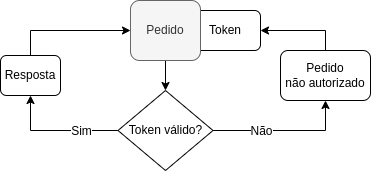
\includegraphics[width=0.5\textwidth]{images/implementacao/api/jwt_session.png}
  \caption{Utilização de tokens}
  \label{fig:64}
\end{figure}

A grande valia da utilização da técnica de autenticação mencionada anteriormente é a segurança. Isto acontece porque estes \textit{tokens} têm geralmente uma duração muito curta como por exemplo quinze minutos, e sempre que um \textit{token} de sessão expira o utilizador necessita de realizar novamente o login, o que poderá tornar a utilização da aplicação imprática.

A solução deste problema sem a perda de segurança significativa veio pelo meio da utilização de \textit{tokens} de duração maior em conjunto com os \textit{tokens} de duração curta. Enquanto o \textit{token} de grande duração se encontrar válido, novos \textit{tokens} de curta duração são gerados para o utilizador, o que leva a que o utilizador nunca perca a sua sessão. Estes \textit{tokens} de grande duração têm por nome \textit{refresh tokens} e os \textit{tokens} de curta duração têm por nome \textit{session tokens}. Sempre que o utilizador termina a sua sessão o \textit{refresh tokens} deverá ser apagado.

Sempre que um utilizador realiza um pedido,o seu \textit{token} de sessão deverá ser validado, caso este seja válido, o seu \textit{refresh token} deverá também ser validado e apenas após esta verificação o utilizador estará autenticado. Na eventualidade de o \textit{token} de sessão ou de \textit{refresh} se encontrarem expirados, este a estará sem autorização para realizar o pedido, mas poderá pedir um novo \textit{token} de sessão enquanto o seu \textit{refresh token} estiver válido, isto acontece sem realizar novamente o \textit{login} e sem o utilizador perceber.

 Além das funcionalidades atrás mencionadas é possível também associar dados em formato \textit{json} a um \textit{token jwt}, esta funcionalidade foi utilizada para enviar o \textit{id} e cargo do utilizador a qual pertence este \textit{token}.

 \newpage

\subsubsection{Validação de Papel}

Com finalidade de garantir que apenas empresas podem realizar os pedidos de empresas e apenas técnicos e empresas podem realizar os pedidos de técnicos foi então criado um middleware que valida se o utilizador que realizou o pedido tem permissões para o mesmo. Este middleware interliga-se com o middleware anterior pois como mencionado o cargo do utilizador em questão é enviado no token, sendo assim é obtido este cargo e realizada uma comparação, com o cargo desejado. Para isto foram criados 2 middlewares diferentes, um valida o cargo de empresas e o outro o cargo de técnicos. Visto que as empresas podem realizar operações de técnicos então no middleware de técnicos é verificado se o token corresponde a um utilizador empresa ou a um utilizador técnico, já no middleware de validação de empresa é verificado se o utilizador tem cargo de empresa.


% //TODO : Adicionar esquema a mostrar como estes middlewares funcionam
